\section{Введение}

\textbf{Цель работы:}
определить скорость полета пули, применяя законы сохранения и используя баллистические маятники.

\textbf{В работе используются:}
духовое ружье на штативе, осветитель, оптическая система для измерения отклонений маятника, измери-тельная линейка, пули и весы для их взвешивания, а также балли-стические маятники.


Скорость вылета пули из духового ружья 150-200 м/с, из боевой винтовки ~1000 м/с.

Это скорости большие по сравнению, скажем, со скоростью пешехода (~2 м/с) или даже автомобиля (~20 м/с). Поскольку размер лабораторной установки обычно порядка нескольких метров, время пролета пули составляет величину порядка $10^{-2}-10^{-3}$ с. Для измерения таких величин необходима дорогостоящая аппаратура, регистрирующая быстропеременные процессы. Дешевле определить скорость пули по импульсу, передаваемому ею некоторому телу при неупругом соударении. В отсутствие внешних сил, а при кратковременном ударе даже и при действии внешних сил, импульс системы пуля-тело сохраняется. Если масса тела значительно больше массы пули, то скорость тела с застрявшей в нем пулей будет значительно меньше скорости пули, и ее легче измерить. Длительность неупругого соударения пули и тела, измеряемая с момента их соприкосновения до прекращения относительного движения, зависит от сопротивления, которое испытывает пуля при движении внутри тела. Оценить ее можно по глубине проникновения пули в тело, предполагая силу сопротивления постоянной.

Если при скорости 200 м/с глубина проникновения ~1 см, то время соударения $~10^{-4}$ с. За это время даже тело только в 100 раз более тяжелое, чем пуля, сдвинется всего на 0,1 мм. При малых временах соударения внешние силы конечной величины сообщают импульс, намного меньший импульса пули.

В ходе работы будут применены законы сохранения импульса:
\[\sum \vec{p} = \sum \vec{p'}\]
и закон сохранения момента импульса:
\[\sum \vec{L} = \sum \vec{L'}.\]

\subsection{Баллистический маятник, совершающий поступательное движение}

Используемый в этой работе баллистический маятник представляет собой тяжелый цилиндр, подвешенный на четырех нитях одинаковой длины. Он изображен на рис. 1 вместе с измерительной системой. Важной особенностью используемой системы подвески маятника является то, что при колебаниях ось цилиндра перемещается параллельно самой себе без вращения. Колебания происходят так, как будто вся масса маятника сосредоточена в его центре масс. Любая точка цилиндра при колебаниях маятника движется по дуге окружности, радиус которой равен расстоянию по вертикали между уровнями верхнего и нижнего концов нитей подвеса.

\begin{figure}[H]
    \centering
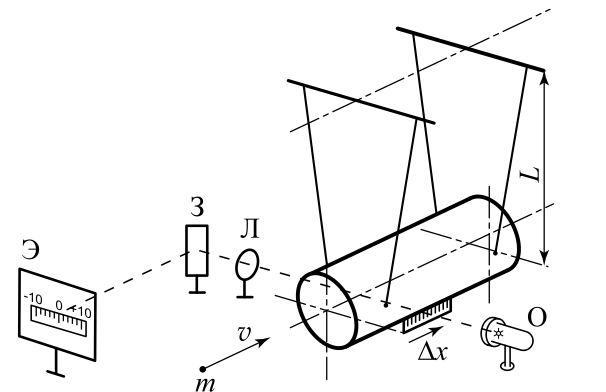
\includegraphics[width=1.\linewidth,center]{p1.png}
    \caption{Схема установки для измерения скорости полета пули с баллистическим маятником, совершающем поступательное движение}
    \label{fig:my_label}
\end{figure}

Связь между максимальным отклонением маятника и начальной скоростью, полученной им в результате толчка, описывается законом сохранения механической энергии, если потери энергии за период значительно меньше энергии его колебаний. По начальному максимальному отклонению маятника определяются импульс и скорость пули.

\newpage
\subsection{Крутильный маятник}

Схема эксперимента изображена на рис. 2. Пуля массой $m$
попадает в мишень, укрепленную на стержне $aa$, который вместе
с грузами $М$ и проволокой П образует крутильный маятник.
Считая удар пули о мишень неупругим, для определения скорости
и полета пули непосредственно перед ударом воспользуемся
законом сохранения момента импульса в виде
\[mur = I\Omega.\]
\begin{figure}[H]
    \centering
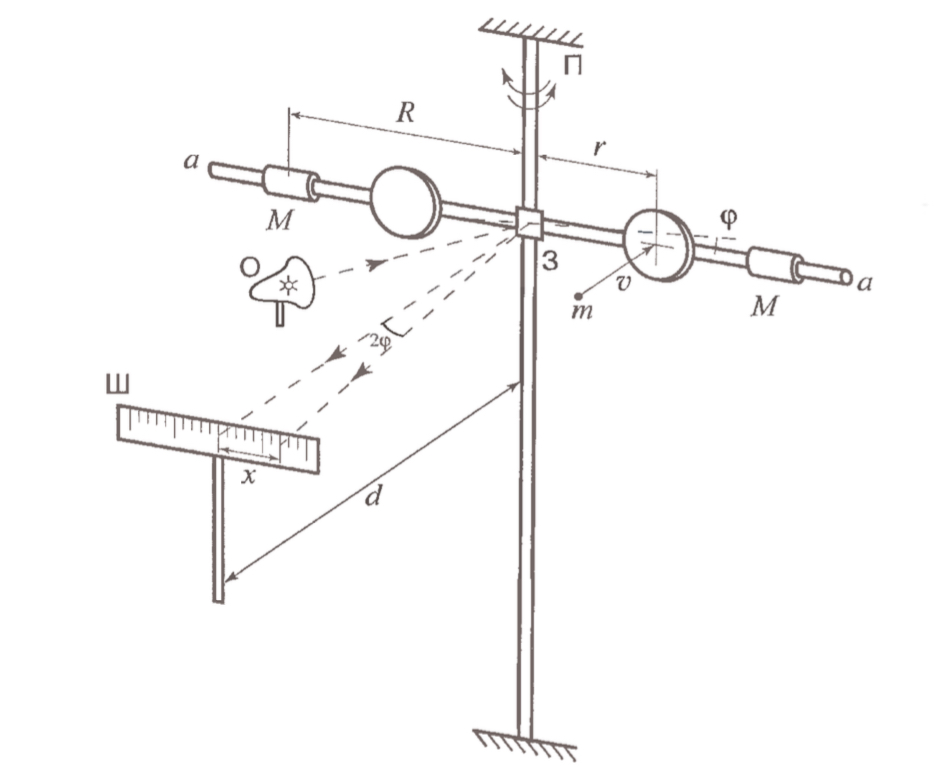
\includegraphics[width=1.\linewidth,center]{p2.jpeg}
    \caption{Схема установки для измерения скорости пули с крутильным баллистическим маятником}
    \label{fig:my_label}
\end{figure}
Здесь $r$ — расстояние от линии полета пули до оси вращения
маятника (до проволоки П), $I$ — момент инерции маятника,
$\Omega$ — его угловая скорость непосредственно после удара.

Законом сохранения момента импульса можно воспользоваться, если
время соударения пули с мишенью значительно меньше периода малых
колебаний маятника. Поворот маятника за время соударения мал по
сравнению с максимальным поворотом маятника при колебаниях.
Соответственно мал момент кручения, возникающий при этом в
проволоке, по сравнению с моментом при максимальном повороте,
который всегда, имеет конечную величину. Но главное - мало
произведение момента кручения в проволоке на время соударения
по сравнению с моментом импульса, которым обладала пуля перед
ударом.

Начальная кинетическая энергия вращения маятника переходит в
потенциальную — упругую энергию закручивания проволоки и
расходуется на необратимые потери - в первую очередь на трение о
воздух. Роль потерь можно оценить по изменению амплитуды
колебаний за 10 периодов. Если амплитуда уменьшается менее чем
наполовину, то затухание колебаний считаем малым, то есть
потери энергии за период колебаний значительно меньше
энергии колебаний. Пренебрегая потерями, закон сохранения
энергии при колебаниях записываем следующим образом:

\[k\frac{\varphi^2}{2} = I\frac{\Omega^2}{2}.\]

Здесь $k$ -- модуль кручения проволоки П, а $\varphi$ --
максимальный угол поворота маятника.

Из ЗСЭ и ЗСМИ получаем:
\[u = \varphi\frac{\sqrt{kI}}{mr}\]

Период колебаний с грузами и без них:

\[T_1 = 2\pi\sqrt\frac Ik,\]
\[T_2 = 2\pi\sqrt\frac{I - \left(M_1+M_2\right)R^2}{k}.\]
Следовательно,
\[\sqrt{kI} = \frac{2\pi\left(M_1+M_2\right)R^2T_1}{T_{1}^2 - T^{2}_2}.\]
